\section{Introduction}
\begin{frame}{\VideoName}
    \tableofcontents[currentsection]
\end{frame}

\begin{frame}{Non-profiled SCA}
    \begin{itemize}
        \item If the attacker does not have access to a similar device, just the target device or just the measurements coming from the target device, we talk about a \textit{non-profiled SCA}.
        \item In a general scenario, this attack utilizes a set of traces where a fixed secret key is used to encrypt multiple (random) plaintexts.
    \end{itemize}
\end{frame}

\begin{frame}{Profiled SCA}
    \begin{itemize}
        \item If we assume the attacker has access to a clone device of the target device, then the attacker can carry out a \textit{profiled SCA}.
       \item The attack operates in two phases.
        \item In the profiling phase, the attacker acquires side-channel measurements for known plaintext/ciphertext and known key pairs.
       \item This set of data is used to characterize or model the device.
        \item Then the attacker acquires a few measurements from the target device, usually identical to the clone device, with known plaintext/ciphertext but the key is secret.
        \item These measurements from the target device are then tested against the characterized model from the clone device.
    \end{itemize}
\end{frame}

\begin{frame}{Datasets}
There are two datasets that will be analyzed in more detail in this video.

Both datasets
\begin{itemize}
    \item Capture one round of software implementation of PRESENT.
    \item \texttt{nop} operations before and after PRESENT computation
    \item Each trace has $3600$ time samples
\end{itemize}
More details on individual datasets:
\begin{itemize}
    \item \dataranone: This dataset contains 5000 traces with a fixed round key \texttt{0xFEDCBA0123456789} and a random plaintext for each trace --\textbf{attack dataset}
    \item \datarantwo: This dataset contains 10000 traces with a random round key and a random plaintext for each trace -- \textbf{profiling dataset}
\end{itemize}
\end{frame}

\section{Profiled DPA Attack Steps}
\begin{frame}{\VideoName}
    \tableofcontents[currentsection]
\end{frame}

\begin{frame}{Profiling phase}
    \begin{itemize}
        \item Suppose the \datarantwo is obtained from a clone device -- \textit{profiling traces}
        \item The \dataranone is from the target device -- \textit{attack traces}
        \item Before the attack, we can analyze \datarantwo to obtain more information about the leakage behavior of the devices -- \textit{profiling phase}.
        \item The first major step in the profiling phase is to find the POIs -- time samples that will give us more information, or with better signal.
        \item Instead of computing the sample correlation coefficients for all time samples, we can just focus on the POIs.
    \end{itemize}
\end{frame}

\begin{frame}{Attacker assumption}
    \begin{itemize}
        \item The attacker has the knowledge of the plaintext and the goal is to recover the very first round key of a symmetric block cipher -- for some
ciphers, e.g. PRESENT, this is the first round key; for some ciphers, e.g. AES, this is the whitening key, which is equal to the master key..
        \item Similar attack strategies apply if we assume the attacker has the knowledge of the ciphertext and aims to recover the last round key.
        \item We also assume the attacker has the knowledge of the detailed implementation so that the same program can be implemented by the attacker on the clone device.
        \begin{itemize}
            \item This is different from the non-profiled setting where only certain basic knowledge of the implementation is required -- For example, how to interface with the encryption routine, whether the computation is executed serially or in parallel, or whether some types of countermeasures are present.
        \end{itemize}
    \end{itemize}
\end{frame}

\begin{frame}{Profiled DPA -- step 1}
\textbf{Identify the target cryptographic implementation}
    \begin{itemize}
        \item Profiled DPA attacks can be applied to unprotected implementations of any symmetric block cipher that has been proposed so far.
    \end{itemize}
    \begin{example}
        As a running example, we will look at the computation of PRESENT.
    \end{example}
\end{frame}

\begin{frame}{PRESENT -- encryption}
\begin{columns}[T] % align columns
\begin{column}{.55\textwidth}
\begin{itemize}
     \item block length: $n=64$
       \item number of rounds: \texttt{Nr}$=31$
       \item key length: either $80$ or $128$.
    \item Round function: addRoundKey, sBoxLayer, and pLayer.
    \item After $31$ rounds, addRoundKey is applied again before the ciphertext output 
\end{itemize}
\begin{alertblock}{Remark}
    For PRESENT specification, we consider the $0$th bit of a value as the rightmost bit in its binary representation.
For example, the $0$th bit of $3=011_2$ is $1$, the $1$st bit is $1$ and the $2$nd bit is $0$.
\end{alertblock}
\end{column}%
\hfill%
\begin{column}{.5\textwidth}
\begin{figure}
    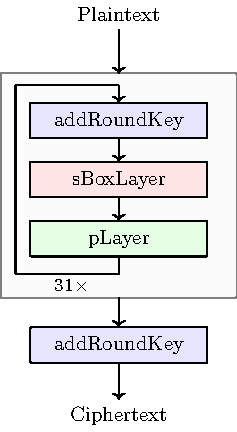
\includegraphics[width=0.6\textwidth]{fig/PRESENT.pdf}
\end{figure}
\end{column}%
\end{columns}
\end{frame}

\begin{frame}{Two rounds of PRESENT}
    \begin{itemize}
        \item For our DPA attacks, we will attack the $0$th Sbox and try to recover one nibble of the first round key
    \end{itemize}
    \begin{figure}
    \centering
    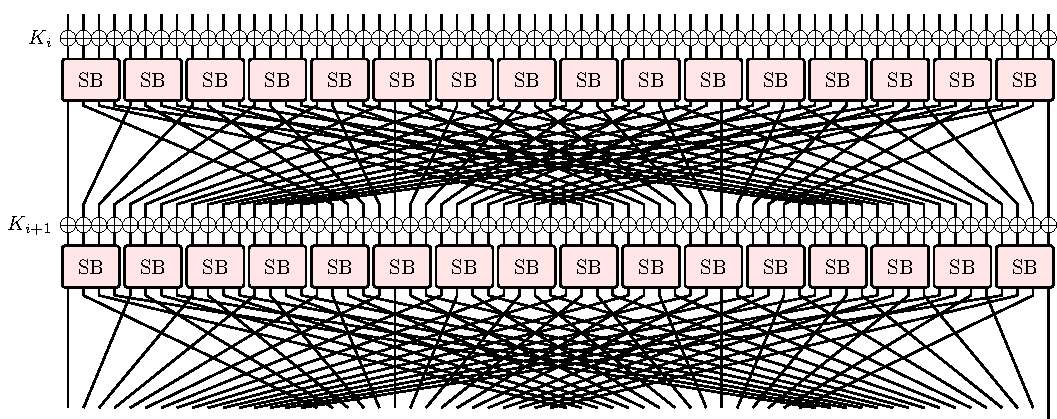
\includegraphics[width=0.9\textwidth]{fig/PRESENT_two_rounds.pdf}
\end{figure}
\end{frame}

\begin{frame}{Profiled DPA -- step 2}
    \textbf{Measurement of profiling traces}
    \begin{itemize}
        \item We first collect a set of traces for profiling using the clone device with random plaintexts and random keys.
        \item Suppose there are in total $M_{pf}$ profiling traces and each trace contains $q$ time samples.
    \end{itemize}
    \begin{example}
    \begin{itemize}
        \item  For our illustrations, we will use the \datarantwo as profiling traces
        \item This dataset contains 10000 traces with a random round key and a random plaintext for each trace.
        \item Each trace has $3600$ time samples
        \item Then $M_{pf}=10000$, and $q=3600$.
    \end{itemize}
    \end{example}
\end{frame}

\begin{frame}{Profiled DPA -- step 3}
    \textbf{Choose the part of the key to recover}
    \begin{itemize}
        \item DPA attack is normally carried out in a divide-and-conquer manner.
       \item We focus on a small part (e.g. a nibble, a byte) of a round key in each attack and each part of the round key can be recovered independently.
       \item With the inverse key schedule, one (e.g. AES) or two round keys (e.g. PRESENT, DES) will reveal the master key
      \item Let $k$ denote the target part of the key and let $M_k$ denote the number of possible values of $k$.
    \end{itemize}
    \begin{example}
        For our attack example, we will focus on the $0$th nibble of the first round key for PRESENT and $M_k=16$.
    \end{example}
\end{frame}

\begin{frame}{Profiled DPA -- step 4}
    \textbf{Choose the target intermediate value}
    \begin{itemize}
        \item To recover the key, we exploit relationships between leakages and a certain intermediate value being processed in the DUT.
       \item The goal is to gain information about this intermediate value, which reveals information about our chosen part of the key.
      \item  Let $\boldsymbol{v}$ denote the target intermediate value.
   \item We require that there is a function $\varphi$, such that
    \[
    \boldsymbol{v}=\varphi(k,p),
    \]
    where $p$ denotes (part of) the plaintext.
    \end{itemize}
    \begin{example}
    \begin{itemize}
        \item $k$: $0$th nibble of the first round key
        \item $\boldsymbol{v}$: $0$th Sbox output of the first round
        \item $p$: $0$th nibble of the plaintext
    \end{itemize}
    \[
    \boldsymbol{v}=\text{SB}_{\text{PRESENT}}(k\oplus p),
    \]
    \end{example}
\end{frame}

\begin{frame}{Profiled DPA -- step 5}
    \textbf{Decide on the target signal}
    \begin{itemize}
        \item Before we do further analysis of the profiling traces, we need to choose what information related to the target intermediate value $\boldsymbol{v}$ we are looking for.
        \item For example, the Hamming weight of $\boldsymbol{v}$; or the $0$th bit of $\boldsymbol{v}$
    \end{itemize}
    \begin{example}
    In our running example, we will look at two types of target signals
        \begin{itemize}
            \item The exact value of $\boldsymbol{v}$
            \item $\wt{\boldsymbol{v}}$, the Hamming weight of $\boldsymbol{v}$.
        \end{itemize}
    \end{example}
\end{frame}

\begin{frame}{Profiled DPA -- step 6}
    \textbf{Compute SNR and identify the POI}
    \begin{itemize}
        \item Compute SNR based on the chosen target signal
        \item We would like to focus on the time sample where the corresponding SNR is the highest.
    \end{itemize}
    \begin{example}
        \begin{itemize}
            \item Signal is given by exact value of $\boldsymbol{v}$
        \begin{itemize}
             \item $\text{POI}=392$.
        \end{itemize}
        \item Signal is given by the Hamming weight of $\boldsymbol{v}$
        \begin{itemize}
             \item $\text{POI}=392$.
        \end{itemize}
        \end{itemize}
    \end{example}
\end{frame}

\begin{frame}{SNR -- exact value}
     \begin{figure} 
        \centering
        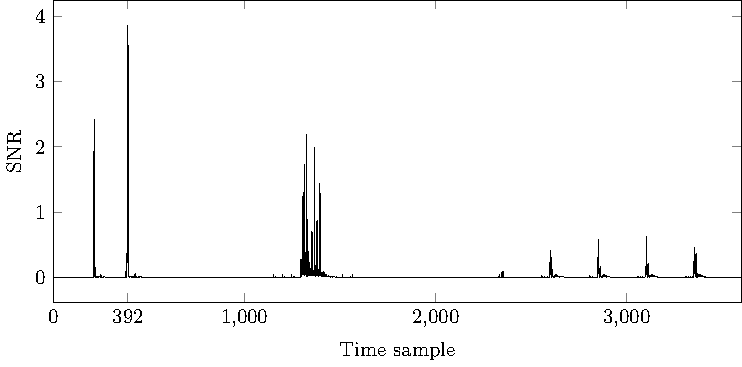
\includegraphics{fig/SNR_identity_model.pdf}
        \caption{
        The signal is given by the exact value of the $0$th Sbox output.
        $\text{POI}=392$}
    \end{figure}
\end{frame}

\begin{frame}{SNR -- Hamming weight}
    \begin{figure} 
        \centering
        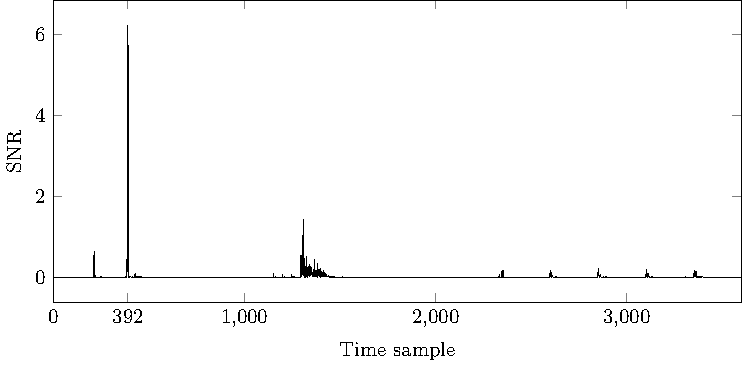
\includegraphics{fig/SNR_hw.pdf}
        \caption{
        The signal is given by the Hamming weight of the $0$th Sbox output.
        $\text{POI}=392$}
    \end{figure}
\end{frame}

\begin{frame}{Profiled DPA -- step 7}
    \textbf{Measurement of attack traces}
    \begin{itemize}
        \item After getting our POI, we are ready to carry out the attack.
         \item The efficiency and success of the attack are highly dependent on the measurement devices the attacker has access to.
        \item Suppose we have taken measurements of our target device with $M_p$ plaintexts.
        \item For $j=1,\dots,M_p$, let $\boldsymbol{\ell}_j$ denote the corresponding power trace, where $q$ is the total number of time samples in one attack trace.
    \end{itemize}
     \begin{example}
        \begin{itemize}
            \item We will use the \dataranone as illustrations.
            \begin{itemize}
                \item Each trace has $3600$ time samples
                \item Contains 5000 traces with a fixed round key \texttt{0xFEDCBA0123456789} and a random plaintext for each trace.
            \end{itemize}
            \item In particular, we have $M_p=5000$, $q=3600$.
        \end{itemize}
    \end{example}
\end{frame}

\begin{frame}{Profiled DPA -- step 8}
    \textbf{Compute hypothetical target intermediate values}
    \begin{itemize}
        \item For each key hypothesis $\hat{k}_i$ of $k$, and each (part of the) plaintext $p_j$, we can compute a hypothesis for $\boldsymbol{v}$:
    \[
    \hat{\boldsymbol{v}}_{ij}=\varphi(\hat{k}_i,p_j),\quad i=1,2,\dots,M_k,\quad j=1,2,\dots,M_p.
    \]
    \end{itemize}
    \begin{example}
        \begin{itemize}
            \item With each key hypothesis of $k$, we have a hypothetical value for $\boldsymbol{v}$:
        \[
    \hat{\boldsymbol{v}}_{ij}=\text{SB}_{\text{PRESENT}}(\hat{k}_i\oplus p_j),\quad i=1,2,\dots,16,\quad j=1,2,\dots,5000.
    \]
    \item $p_j$ is the $0$th nibble of the plaintext corresponding to the attack trace $\boldsymbol{\ell}_j$.
    \item $\hat{k}_i=i-1,\quad i=1,2,\dots,16.$
        \end{itemize}
    \end{example}
\end{frame}

\begin{frame}{Profiled DPA -- step 8}
    \textbf{Compute hypothetical target intermediate values}
    \begin{table}[htb]
\centering
\ttfamily
\begin{tabular}{cccccccccccccccc}\hline
 0 & 1 & 2 & 3 & 4 & 5 & 6 & 7 & 8 & 9 & A & B & C & D & E & F \\\hline
 C & 5 & 6 & B & 9 & 0 & A & D & 3 & E & F & 8 & 4 & 7 & 1 & 2\\\hline
\end{tabular}
\end{table}
    \begin{example}
    \[
    \hat{\boldsymbol{v}}_{ij}=\text{SB}_{\text{PRESENT}}(\hat{k}_i\oplus p_j),\quad i=1,2,\dots,16,\quad j=1,2,\dots,5000.
    \]
    \begin{itemize}
    \item $\hat{k}_1=\texttt{0}$, $\hat{k}_2=\texttt{1}$.
    \item $p_1=\texttt{9},\quad p_2=\texttt{C}.$
    \end{itemize}
      \begin{eqnarray*}
        \hat{\boldsymbol{v}}_{11}&=&\text{SB}_{\text{PRESENT}}(\hat{k}_1\oplus p_1)=\text{SB}_{\text{PRESENT}}(\texttt{0}\oplus\texttt{9})=\text{SB}_{\text{PRESENT}}(\texttt{9})=\texttt{E},\\
        \hat{\boldsymbol{v}}_{12}&=&\text{SB}_{\text{PRESENT}}(\hat{k}_1\oplus p_2)=\text{SB}_{\text{PRESENT}}(\texttt{0}\oplus\texttt{C})=\text{SB}_{\text{PRESENT}}(\texttt{C})=\texttt{4},\\
        \hat{\boldsymbol{v}}_{21}&=&\text{SB}_{\text{PRESENT}}(\hat{k}_2\oplus p_1)=\text{SB}_{\text{PRESENT}}(\texttt{1}\oplus\texttt{9})=\text{SB}_{\text{PRESENT}}(\texttt{8})=\texttt{3},\\
         \hat{\boldsymbol{v}}_{22}&=&\text{SB}_{\text{PRESENT}}(\hat{k}_2\oplus p_2)=\text{SB}_{\text{PRESENT}}(\texttt{1}\oplus\texttt{C})=\text{SB}_{\text{PRESENT}}(\texttt{D})=\texttt{7}.
    \end{eqnarray*}
    \end{example}
\end{frame}

\begin{frame}{Leakage model}
    \begin{itemize}
        \item Assume a value $\boldsymbol{v}$ is being processed in the DUT
        \item Let $\text{noise}\sim\mathcal{N}(0,\sigma^2)$ be a normal random variable with mean $0$ and variance $\sigma^2$.
        \item \textit{identity leakage model}
        \begin{itemize}
            \item the leakage is correlated to $\boldsymbol{v}$
           \[
\mathcal{L}(\boldsymbol{v})=\boldsymbol{v}+\text{noise}.
\]
        \end{itemize}
        \item \textit{Hamming weight model}
        \begin{itemize}
            \item the leakage will then be correlated to $\wt{\boldsymbol{v}}$, the Hamming weight of $\boldsymbol{v}$\footnote{the Hamming weight of vector $\boldsymbol{v}\in\FF_2^m$ is defined to be the number of $1$s in $\boldsymbol{v}$}
            \[
            \mathcal{L}(\boldsymbol{v})=\wt{\boldsymbol{v}}+\text{noise}.
            \]
        \end{itemize}
    \end{itemize}
        \begin{example}
    $\boldsymbol{v}=\texttt{A}$
    \begin{itemize}
        \item identity leakage model: $\mathcal{L}(\boldsymbol{v})=10+\text{noise}$
        \item Hamming weight leakage model: $\mathcal{L}(\boldsymbol{v})=2+\text{noise}$
    \end{itemize}
    \end{example}
\end{frame}

\begin{frame}{Profiled DPA -- step 9}
    \textbf{Identify the leakage model and compute hypothetical signals}
    \begin{itemize}
        \item By our choice of the target signal, we have a corresponding leakage model.
        \item In our analysis, we will consider the identity leakage model and the Hamming weight leakage model corresponding to the signal given by $\boldsymbol{v}$ and $\wt{\boldsymbol{v}}$ respectively.
        \item For each hypothetical target intermediate value, we can compute the hypothetical signal depending on our leakage model
    \[
    \mathcal{H}_{ij}:=\mathcal{L}(\hat{\boldsymbol{v}}_{ij})-\text{noise},\quad i=1,2,\dots,M_k,\quad j=1,2,\dots,M_p.
    \]
    \end{itemize}
    \begin{example}
        \begin{itemize}
            \item With each key hypothesis of $k$, we have a hypothetical value for $\boldsymbol{v}$:
        \[
    \hat{\boldsymbol{v}}_{ij}=\text{SB}_{\text{PRESENT}}(\hat{k}_i\oplus p_j),\quad i=1,2,\dots,16,\quad j=1,2,\dots,5000.
    \]
    \item Hamming weight leakage model: $\mathcal{H}_{ij}=\wt{\hat{\boldsymbol{v}}_{ij}}$
        \item Identity leakage mode: $\mathcal{H}_{ij}=\hat{\boldsymbol{v}}_{ij}$
        \end{itemize}
    \end{example}
\end{frame}

\begin{frame}{Recall what we computed last week}
Same computations apply here
    \begin{example}
    \begin{itemize}
        \item Aim to recover the $0$th nibble of the first round key for PRESENT encryption, denoted $k$
        \item The target intermediate value is the $0$th Sbox output
        \item Attack traces: \dataranone -- $5000$ measurements, the corresponding $0$th nibble of plaintext is denoted $p_j$
        \item With each key hypothesis of $k$, we have a hypothetical value for $\boldsymbol{v}$:
        \[
    \hat{\boldsymbol{v}}_{ij}=\text{SB}_{\text{PRESENT}}(\hat{k}_i\oplus p_j),\quad i=1,2,\dots,16,\quad j=1,2,\dots,5000.
    \]
    \item With a chosen leakage model, we have a hypothetical signal
    \begin{itemize}
        \item Hamming weight leakage model: $\mathcal{H}_{ij}=\wt{\hat{\boldsymbol{v}}_{ij}}$
        \item Identity leakage mode: $\mathcal{H}_{ij}=\hat{\boldsymbol{v}}_{ij}$
    \end{itemize}
    \end{itemize}
    \end{example}
\end{frame}

\begin{frame}{Profiled DPA -- step 10}
   \textbf{Statistical analysis}
    \begin{itemize}
        \item  For a fixed key hypothesis $\hat{k}_i$, we view the modeled leakage as a random variable $\mathcal{H}_i$ that varies when the plaintext changes.
       \item Take $L_\text{POI}$ to be the random variable corresponding to leakage at the POI
    \item We compute the sample correlation coefficient between $\mathcal{H}_{i}$ and $L_{\text{POI}}$ for each key hypothesis $\hat{k}_i$ ($i=1,2,\dots,M_k$):
    \begin{equation*}
    r^{\hat{M}_p}_{i,\text{POI}}:=\frac{\sum_{j=1}^{\hat{M}_p}(\mathcal{H}_{ij}-\overline{\mathcal{H}_i})(l_{\text{POI}}^j-\overline{l_{\text{POI}}})}{\sqrt{\sum_{j=1}^{\hat{M}_p}(\mathcal{H}_{ij}-\overline{\mathcal{H}_i})^2}\sqrt{\sum_{j=1}^{\hat{M}_p}(l_{\text{POI}}^j-\overline{l_{\text{POI}}})^2}},
    \end{equation*}
    where $\overline{\mathcal{H}_i}$ and $\overline{l_{\text{POI}}}$ are averages of $\mathcal{H}_i$ and $L_\text{POI}$ respectively. And
    \[
    \overline{\mathcal{H}_i} = \frac{1}{\hat{M}_p}\sum_{j=1}^{\hat{M}_p}\mathcal{H}_{ij}.
    \]
    is the average of all hypothetical leakages for the same key hypothesis $\hat{k}_i$
    \item To compute $\overline{l_{\text{POI}}}$, take all the leakages at the POI of all traces and take the average
    \end{itemize}
\end{frame}

\begin{frame}{Profiled DPA -- identity leakage model}
    \begin{figure}[h]
    \centering
    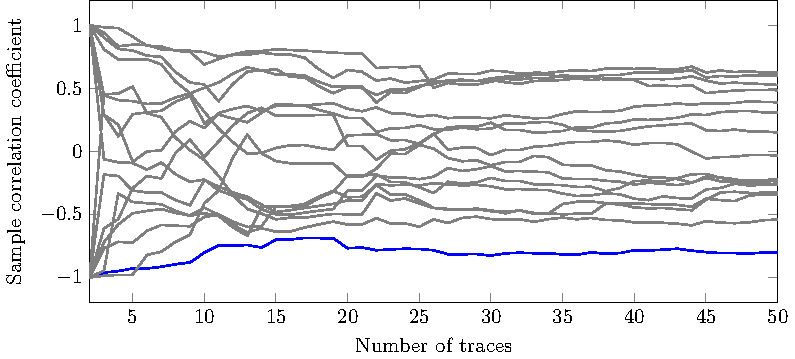
\includegraphics{fig/correlation_POI_identity.pdf}
    \caption{
    $\text{POI}=392$.
    Computed with the \dataranone.
    The blue line corresponds to the correct key hypothesis $\hat{k}_{10}=\texttt{9}$.}
\end{figure}
\end{frame}

\begin{frame}{Profiled DPA -- Hamming weight leakage model}
    \begin{figure}[h]
    \centering
    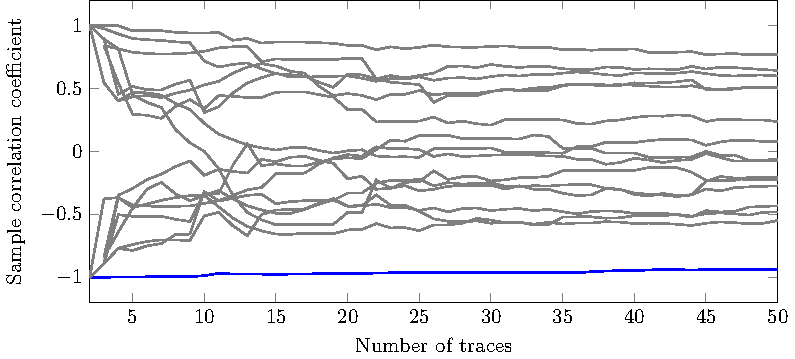
\includegraphics{fig/correlation_POI_hw.pdf}
    \caption{
    $\text{POI}=392$.
    Computed with the \dataranone.
    The blue line corresponds to the correct key hypothesis $\hat{k}_{10}=\texttt{9}$.}
\end{figure}
\end{frame}

\begin{frame}{Nonprofiled DPA from last video}
    \begin{figure}[h]
    \centering
    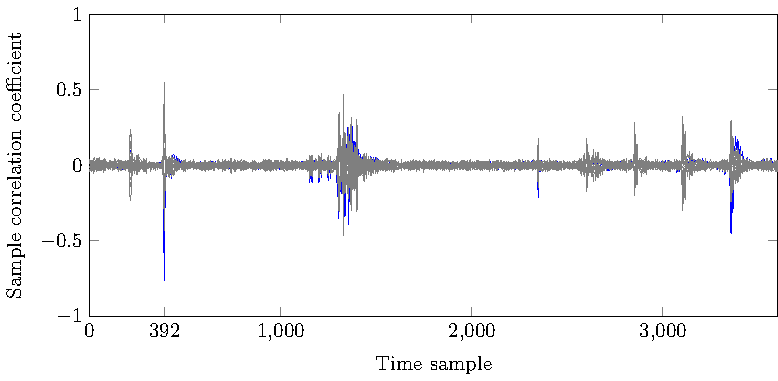
\includegraphics{fig/correlation_coefficients.pdf}
    \caption{Sample correlation coefficients for all $3600$ time samples and all $16$ key hypotheses.
    Computed with the identity leakage model and \dataranone.
    The blue line corresponds to the correct key hypothesis $\hat{k}_{10}=\texttt{9}$.}
\end{figure}
\end{frame}

\begin{frame}{Observations}
    \begin{itemize}
        \item The Hamming weight leakage model is closer to our DUT leakage compared to the identity leakage model
        \item \textit{A good leakage model is beneficial to our attack.}
    \end{itemize}
\end{frame}


\section{Further Reading}
\begin{frame}{\VideoName}
    \tableofcontents[currentsection]
\end{frame}

\begin{frame}{Stochastic leakage model}
    \begin{itemize}
        \item To fully utilize the cloned device in the profiled setting, we can further characterize the leakages instead of just identifying the POI.
        \item Stochastic leakage model: assumes each bit of the target intermediate value has a different leakage.
        \item The attack with stochastic leakage model follows the same steps as described before.
        \item The only difference is in Step 9, where we need extra effort to find our leakage model by profiling.
    \end{itemize}
\end{frame}


\begin{frame}{Template attacks}
    \begin{itemize}
        \item Stochastic leakage model characterizes the leakage assuming each bit of the target intermediate value leaks differently focusing on one POI.
        \item We can also characterize/profile the leakages of each possible value of the target intermediate value at several POIs.
        \item The result of this profiling process is a set of \textit{templates}.
        \item Then during the attack phase, instead of computing correlation coefficients, we use those templates to see which of them fits better to the measured power trace and deduce a probability for each key hypothesis.
    \end{itemize}
\end{frame}

\begin{frame}{Different ordering of traces}
    \begin{itemize}
        \item A different ordering of the traces in \dataranone may affect our attack results.
        \item For example, if arrange the traces in \dataranone in reverse order, we get different results
    \end{itemize}
\end{frame}

\begin{frame}{Profiled DPA -- identity model}
     \begin{figure}[h]
    \centering
    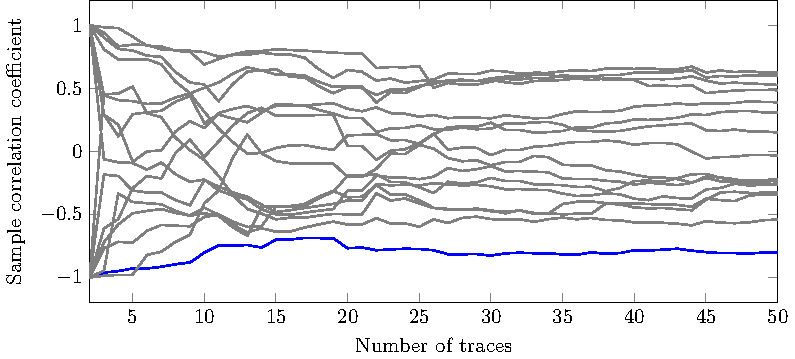
\includegraphics[width=0.6\textwidth]{fig/correlation_POI_identity.pdf}
\end{figure}
 \begin{figure}[h]
    \centering
    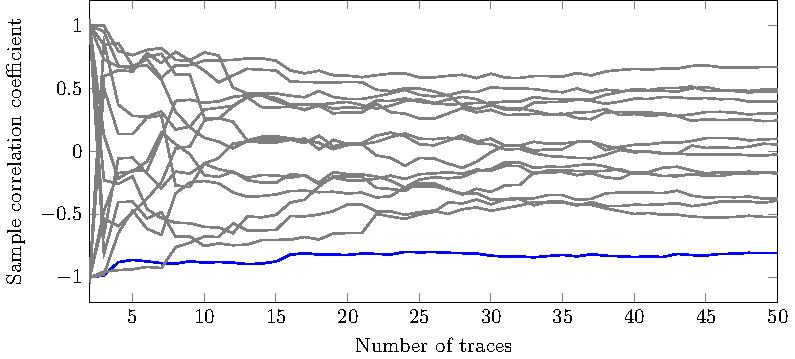
\includegraphics[width=0.6\textwidth]{fig/correlation_POI_identity_reverse.pdf}
\end{figure}
\end{frame}

\begin{frame}{Different ordering of traces}
    \begin{itemize}
        \item To have a fair comparison between different attack methods (e.g. different choices of leakage models, POIs, etc.), \textit{success rate} and \textit{guessing entropy} are used.
    \end{itemize}
    \begin{alertblock}{Remark}
    Our aim is to evaluate the DUT and our implementation against DPA attacks with different settings.
    Thus, we assume we have the knowledge of the key for the evaluation after the attack.
    \end{alertblock}
\end{frame}

\begin{frame}{Key rank}
    \begin{itemize}
        \item For a profiled DPA attack, we assign a \textit{score} to each key hypothesis after the attack: the \textit{absolute value} of the corresponding sample correlation coefficient at POI
        \item Sort the scores in an array in descending order
        \begin{itemize}
            \item Rank $1$st -- highest score
        \end{itemize}
        \item \textit{Key rank} of a key hypothesis: index of the score for the key hypothesis in this sorted array
        \item Ultimate goal of an attack: key rank of the correct key hypothesis $=1$ -- We note that if the key rank is low enough, it is possible to use key enumeration algorithms\footnote{Veyrat-Charvillon, N., Gérard, B., Renauld, M., \& Standaert, F. X. (2013). An optimal key enumeration algorithm and its application to side-channel attacks. In Selected Areas in Cryptography: 19th International Conference, SAC 2012, Windsor, ON, Canada, August 15-16, 2012, Revised Selected Papers 19 (pp. 390-406). Springer Berlin Heidelberg.} that enable the key recovery
        \end{itemize}
\end{frame}

\begin{frame}{Success rate}
    \begin{itemize}
        \item The \textit{success rate} of an attack method with $\hat{M}_p$ traces, denoted SR$_{\hat{M}_p}$, is defined to be 
        \begin{equation*}
       \text{SR}_{\hat{M}_p}=P\left(\text{key rank of the correct key hypothesis}=1\right).
     \end{equation*}
        \item Empirically, we can estimate the value of $\text{SR}_{\hat{M}_p}$ by computing the frequency of $\text{key rank of the correct key hypothesis}=1$ among a certain number of simulated attacks.
    \end{itemize}
\end{frame}

\begin{frame}{Guessing entropy}
    \begin{itemize}
        \item The guessing entropy for an attack method with $\hat{M}_p$ traces is given by the expectation of the key rank of the correct key hypothesis:
\begin{equation*}
    \text{GE}_{\hat{M}_p}=\ex{\text{key rank of the correct key hypothesis with $\hat{M}_p$ traces}}.
\end{equation*}
\item We can approximate $\text{GE}_{\hat{M}_p}$ with the avearged correct key rank among a few simulated attacks.
    \end{itemize}
\end{frame}


\begin{frame}{Success rate -- results}
    \begin{figure}[htb]
    \centering
    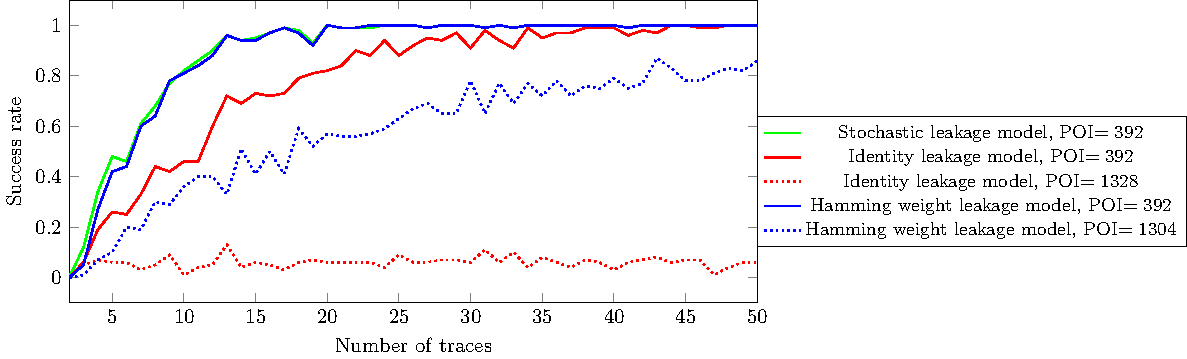
\includegraphics[width=1\textwidth]{fig/SR_DPA.pdf}
\end{figure}
\end{frame}

\begin{frame}{Guessing entropy -- results}
    \begin{figure}[htb]
    \centering
    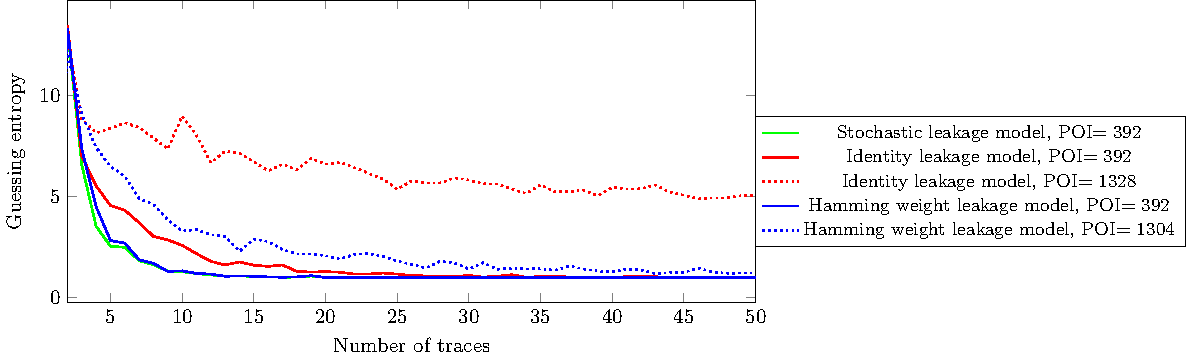
\includegraphics[width=1\textwidth]{fig/GE_DPA.pdf}
\end{figure}
\end{frame}

\begin{frame}{Observations}
    \begin{itemize}
        \item Fewer traces are needed for SR/GE to reach $1$ with the Hamming weight model and stochastic model.
        \item Attack results for the Hamming weight model and stochastic model are similar, with the stochastic model giving slightly better performance.
       \item The choice of POI is important for the attack.
       With the wrong POI, the attack will need much more traces.
    \end{itemize}
\end{frame}

\begin{frame}{Remarks}
    \begin{itemize}
        \item We have discussed SPA on RSA
        \item It is more common to see SPA attacks on public key ciphers and DPA on symmetric key block ciphers
        \item There are also
        \begin{itemize}
            \item DPA on RSA\footnote{Amiel, F., Feix, B., \& Villegas, K. (2007, August). Power analysis for secret recovering and reverse engineering of public key algorithms. In International Workshop on Selected Areas in Cryptography (pp. 110-125). Springer, Berlin, Heidelberg.}
            \item Profiled SPA\footnote{Mangard, S., Oswald, E., \& Popp, T. (2008). Power analysis attacks: Revealing the secrets of smart cards (Vol. 31). Springer Science \& Business Media. Chapter 5}
        \end{itemize}
    \end{itemize}
\end{frame}